\part{Getting started}
\chapter{Installing Tomb Editor}
First of all, you need to download and install the Tomb Editor pack on your computer. wIt is available eg. \href{https://tombengine.com/}{here}.
\par The default route of Tomb Editor installed is \path{C:\Tomb Editor}. The contents of this main folder are:
\begin{itemize}
    \item Tomb Editor program.
    \item Side programs dedicated to Tomb Editor: SoundTool, TombIDE, WadTool.
    \item Most of the files which are necessary to start a basic project and level for Tomb Engine. (But texture files for room faces must be find somewhere else. But this is still not necessary now, when you start reading this tutorial.)
    \item Other important files for Tomb Editor pack.
\end{itemize}
So when you have the Tomb Editor pack installed on your computer, then you are just ready to start building levels for Tomb Engine. \cite{akyv_tutorial}

\chapter{Starting a new project}
After the installation of Tomb Editor pack, you are ready to make your very first Tomb Engine project. (Level map file extensions are well-known as “PRJ” files, but do not misunderstand: what we call “project” now is not a level, but a whole level set - i.e. your current Tomb Engine game itself, which will be released when you fully made it.)
\par But where do you need to place your projects? Well, NOT in Tomb Editor main folder - that is a place you usually never modify while editing. I suggest placing all of your projects nicely collected in a so-called general project folder. This could be called eg. \path{"My_Tomb_Raider_projects"}, created manually. (I created it in Documents folder.)
\par Each project you make will be placed in its own main folder. Does it mean now you should also create manually a project main folder in the general folder? No, there is a TombIDE wizard which will do the whole project-creating procedure for you.
\par Projects are handled in \textbf{TombIDE (Tomb Integrated Development Environment or TIDE)} program, that is why the whole project-creating procedure is also being done there.
So start \path{TombIDE.exe}, and the panel of TIDE Start page opens up.
Click on “Create a new project” button now.
The first page of a new panel opens up (General Information, \ref{fig:tide1}):
\begin{figure}
    \centering
     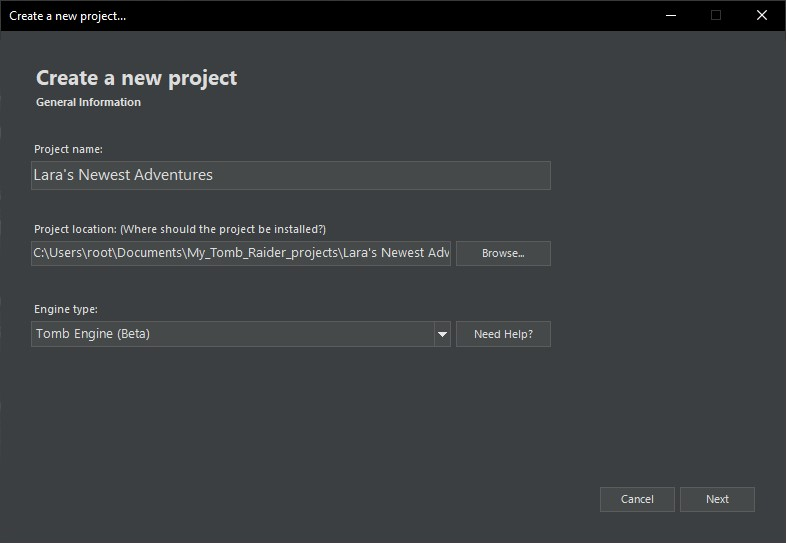
\includegraphics[width=0.75\textwidth]{screenshots/1.jpg}
     \caption{General Information}
     \label{fig:tide1}
\end{figure}

\begin{itemize}
    \item Let's suppose the project you start now has the name of “Lara's Newest Adventures”. So type it now here.
    \item Click on “Browse” button, find and select the general project folder.
    \item After that, the little window in the middle of this first page shows that a subfolder in the general project folder will be created as the main folder of this project, having the project name.
    \item The engine type you choose now is naturally Tomb Engine.
\end{itemize}


\par Now click on “Next” button to continue the procedure on the next page of the panel (Extra Options, \ref{fig:tide2}).

\begin{figure}
    \centering
     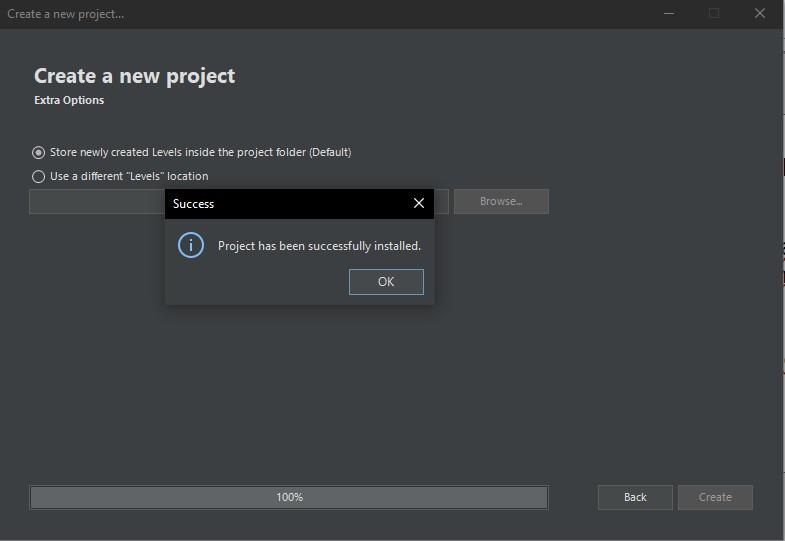
\includegraphics[width=0.75\textwidth]{screenshots/2.jpg}
     \caption{Extra Options}
     \label{fig:tide2}
\end{figure}

\par I suggest changing nothing here. Which means level map files will be handled in a folder called "Levels", which is a subfolder in the main folder of the project. (I mean, this is the default place for level map files, and you, the beginner probably should keep it like this.)
\par Now click on "Create" button here, then look at the increasing bar at the bottom of the panel.
When the bar is at 100 \%, then you get a message that the project has been successfully created (\ref{fig:tide3}).

\begin{figure}
    \centering
     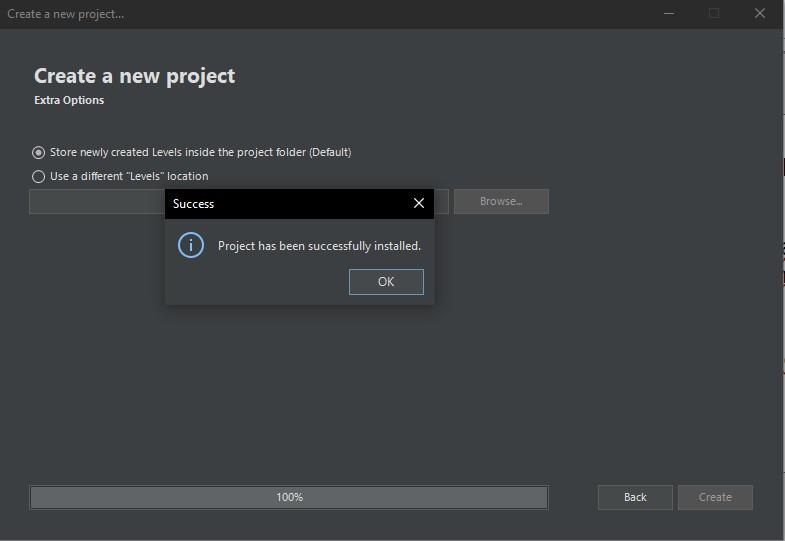
\includegraphics[width=0.75\textwidth]{screenshots/3.jpg}
     \caption{Project has been successfully installed}
     \label{fig:tide3}
\end{figure}

\par And this project main folder has been also created on the selected route, with the basic contents a TEN project should have. (Including Levels folder - still being empty - in that default position., \ref{fig:tide4})

\begin{figure}
    \centering
     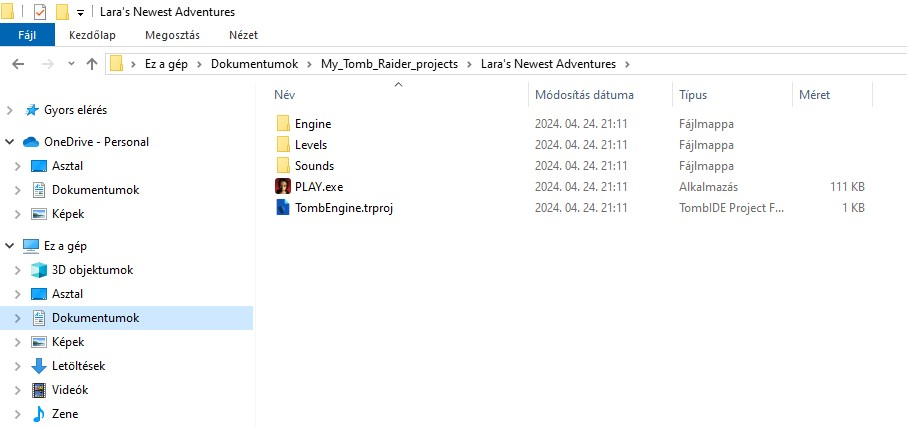
\includegraphics[width=0.75\textwidth]{screenshots/4.jpg}
     \caption{Project directories have been created (Since TEN 1.7., the project main folder has an Assets subfolder as well.)}
     \label{fig:tide4}
\end{figure}

Double-click on that row (or click on "Open selected button" below), so the project opens in TIDE, you will be able to work on it. Each project opened in TIDE has more pages, now you can see its Level Manager page. (See the panel header which names the current project.)
\par Now click on the red arrow in the upper left corner of the page, to go back to TIDE Start page, closing this project now in TIDE. (Since TEN 1.7., you can see the blue TIDE icon in that corner, instead of the red arrow. If you click on that icon, then a menu opens. One of the menu options is an arrow, with "Back to Start Window..." name. Click on it to go back to TIDE Start page.) \cite{akyv_tutorial}